\chapter{Frames: Measuring}\label{app:FrameMeasuring} 
\textbf{Name: Group 630}\\
\textbf{Date: 15/03 - 2016}

%\subsubsection{Purpose}
%Measuring Mass of the Frame and Center of Mass of the Frame.
%
%\subsubsection{Setup}
%\begin{figure}[H]
%  \centering
%	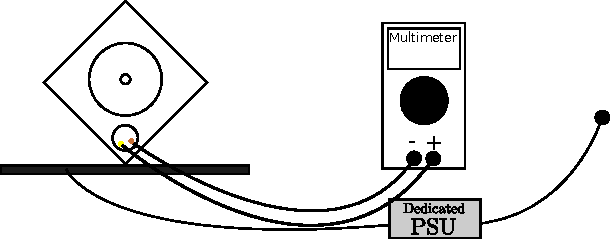
\includegraphics[scale=1]{figures/LabSetupLinearityTest.pdf}
%	\caption{Setup diagram}
%	\label{LabSetupRangeTest}
%\end{figure}\vspace{-5mm}
%
%\subsubsection{List of Equipment}
%\begin{table}[H]
%	\begin{tabular}{|l|l|p{4.3cm}|}
%		\hline%------------------------------------------------------------------------------------------------------------
%		\textbf{Instrument}                                  &  \textbf{AAU-no.}  &  \textbf{Type}                       \\
%		\hline%------------------------------------------------------------------------------------------------------------
%		Multimeter                                           &  60760           &  Fluke 189 Multimeter		                   \\
%		\hline%------------------------------------------------------------------------------------------------------------
%		Dedicated Power Supply of Cubli \small{(24 V - 3 A)} &  AAU3                   &  XP Power, AEB70US24                 \\
%		\hline%------------------------------------------------------------------------------------------------------------
%		Digital Protractor                                   &  None               & CMT Orange Tools     \\
%		\hline%------------------------------------------------------------------------------------------------------------
%	\end{tabular}
%\end{table}
%
%\subsubsection{Procedure}
%\begin{enumerate}
%  \item The Cubli base frame is leveled and the angle of equilibrium point is measured.
%  \item The frame is dismounted from the base frame and weight.
%  \item The frame is mounted back on the base frame after been rotated 90 degrees and the angle of equilibrium point is measured.
%  \item The Cubli frame is returned to original placement on the base frame.
%\end{enumerate}
%
%\subsubsection{Results}
%\begin{table}[H]
%	\begin{tabular}{|l|l|p{4.3cm}|}
%		\hline%------------------------------------------------------------------------------------------------------------
%		\textbf{Frame rotation angle in degrees}       &  \textbf{Angle form equilibrium point in degrees}         \\
%		\hline%------------------------------------------------------------------------------------------------------------
%		0                                & 2,50           \\
%		\hline%------------------------------------------------------------------------------------------------------------
%		90							  & 4,50              \\
%		\hline%------------------------------------------------------------------------------------------------------------
%	\end{tabular}
%\end{table}
%
%\subsubsection{Results}
%\begin{table}[H]
%	\begin{tabular}{|l|l|p{4.3cm}|}
%		\hline%------------------------------------------------------------------------------------------------------------
%		\textbf{Weight of the frame}       &  \textbf{Gram}         \\
%		\hline%------------------------------------------------------------------------------------------------------------
%		 Fully mounted frame        	  & 770          \\
%		\hline%------------------------------------------------------------------------------------------------------------
%	\end{tabular}
%\end{table}	
